\chapter[Разработка приложений с графическим интерфейсом]{Разработка приложений с графическим интерфейсом}
\section[Окна. Класс QMainWindow]{Окна. Класс QMainWindow}
Как уже отмечалось ранее, виджеты, родительский виджет для которых не задан, становятся окнами. Обычно для окон
приложения используют следующие классы:

\begin{itemize}
\item \index{Класс!QMainWindow}\Sys{QMainWindow} --- окно приложения, которое может содержать меню, панели,
строку статуса;
\item \index{Класс!QDialog}\Sys{QDialog} --- диалоговое окно;
\item \index{Класс!QWidget}\Sys{QWidget} --- простое, обычно немодальное окно;
\end{itemize}
Окно обычно имеет обрамление и заголовок. Текст для заголовка окна устанавливают с помощью метода
\Sys{QWidget::setWindowTitle()}. Конструктор класса \Sys{QWidget}
 принимает дополнительный параметр, для типа окна ---
\index{Флаги!Qt::WindowFlags}\Sys{Qt::WindowFlags}. С помощью этого параметра можно
управлять типом обрамления, типом окна (для оконной системы). Например, можно создать окно без обрамления (это полезно
в некоторых случаях для оформления, например, для окна загрузки программы) или деактивировать кнопки для минимизации и
максимизации окна.

\emph{Окно диалога} --- это особый вид окна, который может использоваться для различных
целей, но всегда предоставляет пользователю возможность взаимодействия с программой. Диалоги, как правило, не имеют
кнопок для минимизации и максимизации окна. Окна диалога также часто бывают
\emph{модальными}.
\index{Модальность}\emph{Модальность} окна определяется его поведением.
Модальные окна блокируют доступ к другим окнам, пока пользователь не завершит работу с окном (не закроет его). Задать
модальность окна можно с помощью метода \Sys{QWidget::setWindowModality()}, если
передать ему логическое значение true.

\Sys{QMainWindow} --- класс, реализующий функциональность главного окна приложения. Для этого он дополнительно
имеет специальные средства работы:

\begin{itemize}
\item Главное меню (\EN{Main menu});
\item Панели инструментов (\EN{Toolbars});
\item Панель статуса (\EN{Status bar});
\item Присоединяемые панели (\EN{Docks});
\end{itemize}
Несколько элементов пользовательского интерфейса могут выполнять одно и то же \emph{действие} (например: меню,
кнопка на панели инструментов и т.д.). Класс \index{Класс!QAction}\Sys{QAction} используют для того, чтобы
привязать заданное действие к нескольким элементам управления. Благодаря группировке действия и связанных с ней данных
(названия, подсказки, пиктограммы и т.д.), а также ее многократного использования (в главном меню, на панели
инструментов и т.д.), можно избежать дублирования кода.

\index{Панель!присоединяемая}\emph{Присоединяемые} панели \index{Класс!QDockWidget}\Sys{QDockWidget}
(\EN{dock widgets}), монтируются в крае окна, и могут быть перенесены и перегруппированы
пользователем, или даже разделены и размещены как отдельные окна. Обычно содержат группу элементов пользовательского
интерфейса, объединенных общей целью и назначением или группу инструментов для работы с текущим открытым файлом.

\index{Панель!статуса}\emph{Панель статуса} \index{Класс!QStatusBar}\Sys{QStatusBar}
(\EN{Status bar}) обычно используют для изображения текстовых сообщений о статусе или текущие
действия программы, но она может содержать пиктограммы, а также другие виджеты (например, индикаторы прогресса, метки).

Таким образом, воспользовавшись возможностями главного окна и создав несколько диалогов, можно получить программу,
которая будет соответствовать стандартам современных пользовательских интерфейсов. Сих пор для создания интерфейса
программы нам приходилось самостоятельно создавать и компоновать виджеты. В следующем параграфе мы используем для этой
цели программу \Sys{Qt Designer}, которая позволяет создать интерфейс средствами визуального проектирования.

\section[Быстрая разработка с помощью Qt Designer]{Быстрая разработка с помощью Qt Designer}
Как мы отмечали ранее, есть два подхода, которые можно использовать при построении графического пользовательского
интерфейса, используя виджеты \Sys{Qt}:

\begin{itemize}
\item создать, настроить виджеты и разместить их на форме в соответствующих компоновках с помощью программного кода;
\item воспользоваться визуальным редактором форм \Sys{Qt Designer}, который создаст файл формы (он будет описывать ее внешний
вид, размещение, размеры, настройки, компонование и т.д.). В дальнейшем из файла формы на этапе компиляции будет создан
файл с кодом программы, будет программно создавать этот интерфейс и предоставлять программисту доступ к элементам на
форме.
\end{itemize}
\emph{Файлы }\index{Файл!формы}\emph{формы} имеют расширение \Sys{.ui}. \Sys{Qt Designer} позволяет
редактировать файлы форм, содержащих настройки вида виджетов. \Sys{Qt Designer} можно использовать как отдельную программу
или воспользоваться интеграцией с оболочкой \Sys{Qt Creator} --- редактором форм.

Визуальный \index{Редактор форм}редактор форм позволяет воспользоваться фактически всеми стандартными элементами
управления имеющимися в \Sys{Qt}, настроить значение для их свойств, стилизовать их внешний вид и скомпоновать их на форме.
Также он содержит большое количество инструментов: поле для редактирования формы, редактор сигнально-слотовых
соединений, редактор свойств объектов, средства для работы с компоновками, стилями и~т.~п.

Для того, чтобы продемонстрировать работу редактора форм, создадим новый пример --- простой редактор текста:

\begin{enumerate}
\item Для того, чтобы создать форму главного окна, мы воспользуемся настройками мастера новых проектов. Вызовите мастер
создания файлов и проектов, и выберите тип проекта \Sys{Qt Widgets Application}(Приложение \Sys{Qt Widgets}). 
В окне мастера
введите имя для нового проекта (например: <<\Sys{SimpleTextEditor}>>), выберите также
инструментарий для проекта. В окне \Sys{Class Information} (Информация о классе) выберите
\Sys{QMainWindow} в качестве базового класса главного окна. Также установите флажок \Sys{Generate Form}
(Создать форму) --- это укажет мастеру на необходимость
создания \Sys{.ui}-файла для главного окна (см. рис.~\ref{ch15:refDrawing0}).
\end{enumerate}

\begin{figure}[htb]
\begin{center}
\includegraphics[width=0.7\textwidth]{img/ris_15_1}
\caption[Окно мастера проектов: создание класса главного окна и формы.]{Окно мастера проектов: создание класса
главного окна и формы.}
\label{ch14:refDrawing0}
\end{center}
\end{figure}

\begin{enumerate}
\item После создания проекта откройте дерево проекта, и в разделе \Sys{Forms}(Формы) выберите файл формы для главного окна
(\Sys{mainwindow.ui}). \Sys{Qt Creator} сразу перейдет в режим редактирования пользовательского интерфейса
\Sys{Design }(Дизайн). Интерфейс редактора форм состоит из нескольких панелей (см. рис.~\ref{ch15:refDrawing1}).
\item Выберите на панели виджетов <<\Sys{Plain Text Edit}>> и перетащите его мышкой на
форму. Для удобного поиска виджетов вы можете воспользоваться фильтром в верхней части панели. Для поиска виджета
введите его название.
\begin{figure}[htb]
\begin{center}
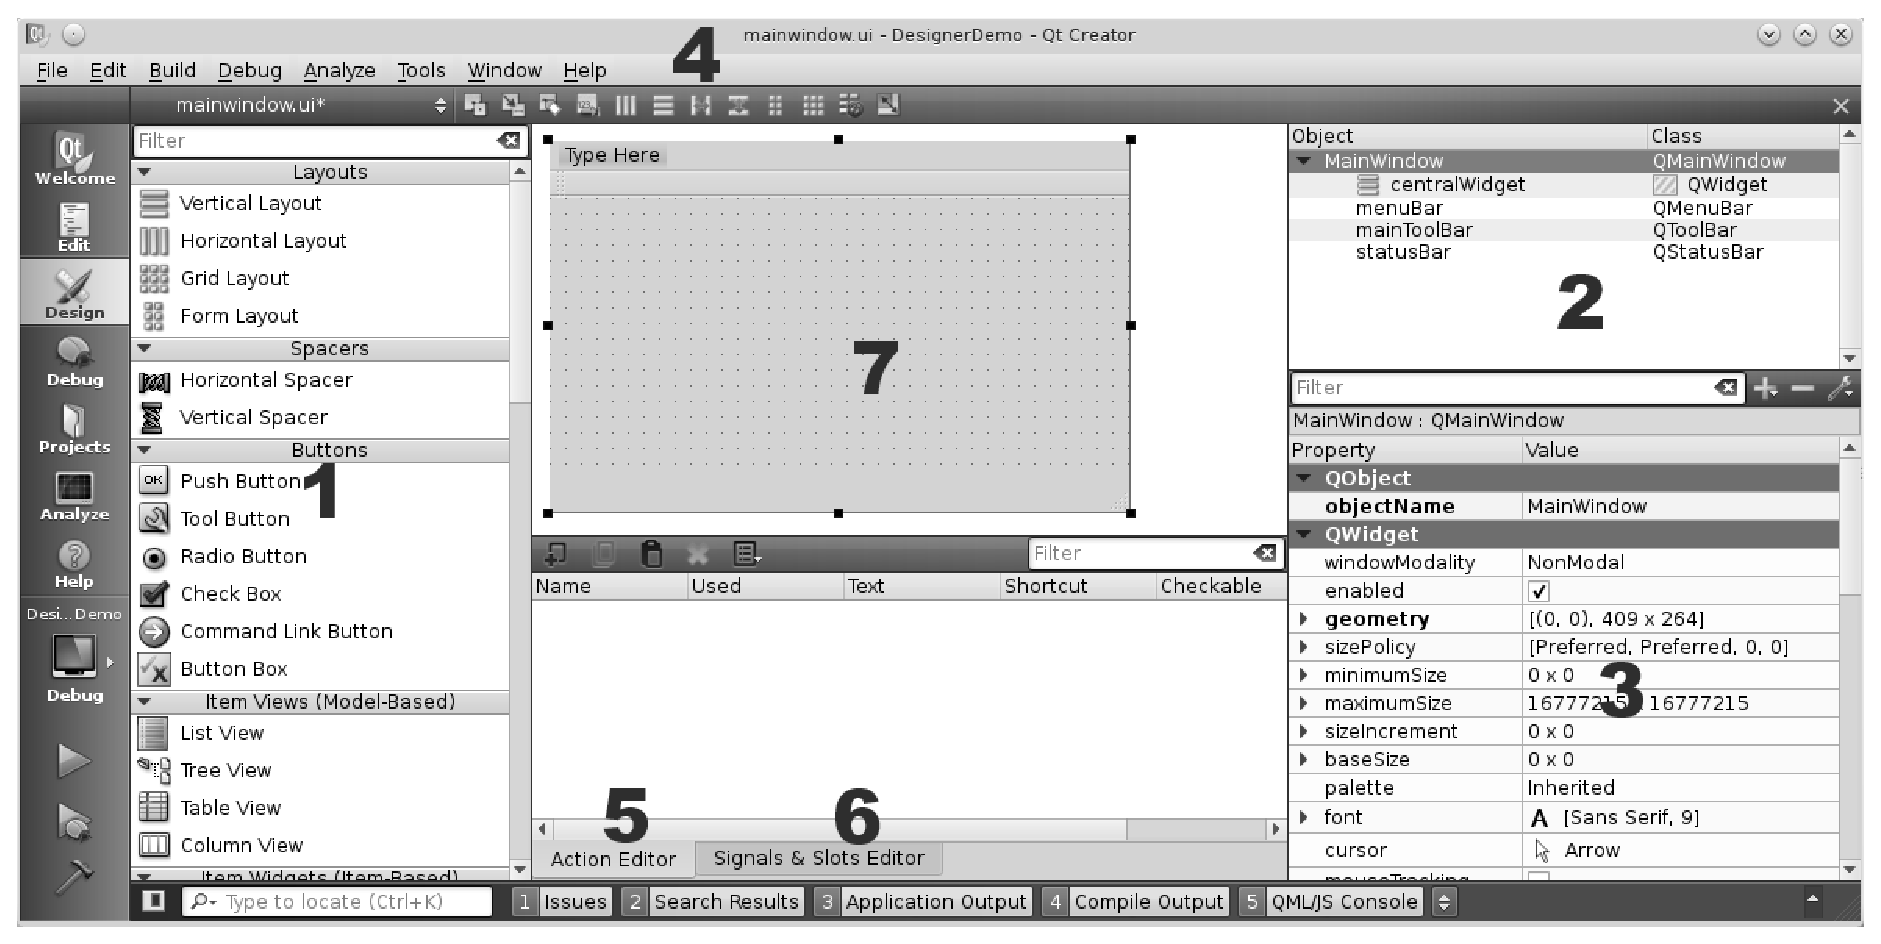
\includegraphics[width=0.8\textwidth]{img/ris_15_2}
\caption[Интерфейс редактора форм.]{Интерфейс редактора форм: 1. Панель виждетов (Widget box) 2. Окно дерева объектов (Object inspector)
3. Редактор свойств (Property editor) 4. Панель переключения режимов работы редактора форм 5. Редактор действий (Action
editor) 6. Редактор сигнально-слотовых соединений (Signals \& Slots editor) 7. Центральная часть окна, в которой
размещена форма.}
\label{ch14:refDrawing0}
\end{center}
\end{figure}

\item Для того чтобы разместить \Sys{Plain Text Edit} в компоновке внутри главного окна, нажмите правой
кнопкой мыши на свободной от виджетов части формы и выберите в контекстном меню тип компоновки (подменю
\Sys{Lay out}). Для примера мы используем вертикальную компоновку. После выбора компоновки текстовое
поле займет все свободное пространство формы.
\item Добавим главное меню программы. Поскольку для главного окна был избран класс \Sys{QMainWindow}, то панель главного меню
(\Sys{QMenuBar}) , панель статуса (\Sys{QStatusBar}) и панель инструментов (\Sys{QToolBar}) автоматически добавлены к проекту (убедитесь
в этом просмотрев дерево объектов). Главное меню расположено в верхней части формы, и пока не содержит ни одного
элемента. Нажмите два раза мышкой на надписи Type here в главном меню, и введите <<\&File>>. По окончании
ввода нажмите Enter --- на форме появится меню <<File>>. Откройте меню <<File>> и введите так же
еще пункты: <<\&New>>, <<\&Open...>> и <<\&Save...>>. Добавьте разделитель в меню
нажав <<Add separator. После этого добавьте еще один пункт --- \Sys{\&Exit.} 
\item Так же добавьте меню <<Edit>> и <<About, добавьте подпункты для этих меню (смотрите на
рисунке ниже). Для того, чтобы к пунктам главного меню можно получить доступ с помощью комбинации клавиш
(Alt+{<}подчеркнутая буква в названии пункта{>}), используют символ <<\&. Например,
для того чтобы открыть меню File с помощью комбинации Alt+F, название пункта меню задают как <<\&File
(см. рис. \ref{ch15:refDrawing3}--\ref{ch15:refDrawing4}). Все пункты меню и разделители можно упорядочить перетащив
мышкой. Дополнительные подменю можно создать для каждого из пунктов меню, которые уже существуют, нажав на значок
справа от названия пункта. 
\end{enumerate}
{\centering\itshape
 
\par}

\begin{figure}[htb]
\centering
 [Warning: Image ignored] % Unhandled or unsupported graphics:
%\includegraphics[scale=0.33]{glava15-img003}
\caption[Меню <<File>> после редактирования..]{Меню <<File>> после редактирования..}

\end{figure}
\begin{figure}[htb]
\centering
 [Warning: Image ignored] % Unhandled or unsupported graphics:
%\includegraphics[scale=0.33]{glava15-img004}
\caption[Меню \ <<Edit>> \ после редактирования]{Меню  <<Edit>>  после редактирования}
\label{ch15:refDrawing3}

\end{figure}
\begin{figure}[htb]
\centering
 [Warning: Image ignored] % Unhandled or unsupported graphics:
%\includegraphics[scale=0.33]{glava15-img005}
\caption[Меню \ <<About>> после редактирования..]{Меню  <<About>> после редактирования..}
\label{ch15:refDrawing4}

\end{figure}
\begin{enumerate}
\item Для каждого из пунктов автоматически было создано соответствующее действие (\index{Класс!QAction}\Sys{QAction}). Список
действий можно просмотреть в редакторе действий (Action editor) на одной из страниц нижней панели редактора форм.
Нажмите два раза мышкой на действие - появится диалоговое окно, в котором можно отредактировать свойства для действия:
текст (Text), имя объекта \Sys{QAction} (Object name), подсказку (ToolTip) --- для панели инструментов, куда будет добавлен
действие, значок (Icon) и комбинацию клавиш для вызова действия (Shortcut). Например, для того, чтобы ввести комбинацию
клавиш, просто нажмите на поле Shortcut и нажмите выбранную комбинацию. Пока мы не будем добавлять горячие комбинации
клавиш. Окончательный вид списка действий после редактирования меню смотрите на рис. \ref{ch15:refDrawing5}унке ниже. 
\end{enumerate}
{\centering  [Warning: Image ignored] % Unhandled or unsupported graphics:
%\includegraphics[scale=0.33]{glava15-img006}
\captionof{figure}[Вид списка действий в редакторе действий (Action Editor) после редактирования меню]{Вид списка
действий в редакторе действий (Action Editor) после редактирования меню}
\label{ch15:refDrawing5}
\par}

\begin{enumerate}
\item Уже на этапе конструирования пользовательского интерфейса в редакторе форм мы можем создать сигнально-слотовые
соединения между объектами на форме. Для этого перейдите на вкладку Signals \& Slots Editor на нижней панели. Для того,
чтобы добавить новое соединение нажмите на значок с символом <<+. Появится новая строка, в которой
двойным щелчком мыши в каждом из столбцов можно вызвать меню со списком доступных вариантов . Выберите в качестве
объекта (Sender) actionExit, который будет посылать сигнал (Signal) triggered(), а в качестве адресата (Receiver)
выберите MainWindow и слот (Slot) close(). Также добавьте остальные сигально- слотовые соединения для действий, как на
рис. \ref{ch15:refDrawing6}.

\end{enumerate}
{\centering  [Warning: Image ignored] % Unhandled or unsupported graphics:
%\includegraphics[scale=0.33]{glava15-img007}
\captionof{figure}[Вид редактора сигнально{}-слотовых соединений (Signals \& Slons Editor) после редактирования]{Вид
редактора сигнально-слотовых соединений (Signals \& Slons Editor) после редактирования}
\label{ch15:refDrawing6}
\par}

\begin{enumerate}
\item Такие действия как Undo (Отменить) , Redo (Повторить) , Cut (Вырезать) , Copy (Копировать), теперь присоединены к
соответствующим сигналам Plain Text Edit, которые будут сигнализировать о возможности их выполнение действий
пользователя в редакторе. Запустим созданную форму в режиме просмотра --- для этого выберите Tools-{>}Form
Editor-{>}Preview... или нажмите комбинацию клавиш (Alt+Shift+R). Редактор форм загрузит и покажет на экране
форму без предварительной компиляции всей программы. Если мы сразу же откроем меню, то увидим что пункты Undo, Redo,
Cut, Copy уже активны, хотя изменения, отмены и выделение текста еще не происходило. Это связано с тем, что по
умолчанию, созданные действия являются активными. Для того чтобы это исправить, откройте дерево объектов (Object Tree),
выберите любую из действий для пунктов Undo, Redo, Cut, Copy и снимите флажок enabled для них в редакторе свойств
(Property Editor). Редактор свойств позволяет настроить каждый из виджетов на форме, изменив значение для их свойств. 
\item Скомпилируйте программу и запустите. Главное окно будет иметь вид, который мы задали на этапе проектирования
формы. Некоторые пункты меню уже работают благодаря сигнально-слотовым соединениям, которые мы сделали.
\end{enumerate}
В следующем параграфе мы продолжим работу над примером и продемонстрируем, как получить доступ к элементам формы из кода
программы.

\section[\ Программирование формы созданной в \Sys{Qt Designer}]{ Программирование формы созданной в \Sys{Qt Designer}}
Рассмотрим, как файлы \index{Файл!формы}форм интегрируются в проект. Как мы уже отмечали ранее, для того чтобы добавить
файл формы в проект существует специальная переменная FORMS. Если мы откроем .рro-файл, то увидим: 

FORMS  += mainwindow.ui

Файлы форм добавленые в проект, считываются и превращаются в эквивалентный С++ код с помощью специальной программы uic
(это происходит во время предварительной обработки проекта с помощью qmake). Код сгенерированный uic создает виджеты и
компоновки, содержит настройки свойств, сигнально-слотовые соединения и стили, необходимые для получения визуального
отображения содержимого .ui-файла. Если мы откроем папку с собранные проектом (или папку для shadow build), то увидим
среди исходных текстов и сгенерированных файлов файл ui\_mainwindow.h, содержащий сгенерированный для формы код.
Конечно, этот файл должен быть добавлен где-то в коде программы с помощью директивы \#include для того, чтобы можно
было воспользоваться сгенерированным кодом. Но нет необходимости делать это самостоятельно --- гораздо легче
воспользоваться мастером создания файлов и проектов. 

При создании проекта для нашего примера мы установили флажок Generate form для того, чтобы автоматически сгенерировать
форму для главного окна и добавить необходимый код для доступа к элементам на форме в программе. Среди кода, мастер
автоматически добавил к объявлению и реализации класса MainWindow: 

\begin{itemize}
\item предварительное объявление класса формы: 
\end{itemize}
\textit{//} \textit{Предварительное} \textit{объявление класса формы}\textit{ }

\textit{//} \textit{созданной с. ui-файла}\textit{ }

namespace Ui \{

 class MainWindow;

\}

\begin{itemize}
\item указатель на объект формы, позволяющий получить доступ к элементам на форме: 
\end{itemize}
class MainWindow : public \Sys{QMainWindow}

\{

.....

private:

 \textit{//} \textit{Указатель на объект формы}\textit{ }

 \textit{//} \textit{созданной с. ui-файла}\textit{ }

 Ui::MainWindow *ui;  

\};

\begin{itemize}
\item Конструктор главного окна создает объект класса формы и инициализирует переменную ui, а также вызывает метод
ui-{>}setupUi(this), который создает все элементы которые есть на форме и устанавливает текущий виджет как
родительский для них; 
\end{itemize}
\textit{//} \textit{Файл сгенерированный uic}\textit{ }

\textit{//} \textit{при обработке файла формы}\textit{ }

\#include \textit{ui\_mainwindow.h}

MainWindow::MainWindow(\Sys{QWidget} *parent) :

 QMainWindow(parent),

 ui(new Ui::MainWindow) \textit{//} \textit{Создаем объект формы}\textit{ }

 \textit{//} \textit{созданной в \Sys{Qt}Designer}\textit{ }

\{  

ui-{>}setupUi(this); \textit{//} \textit{Применяем дизайн, который мы создали в}

\textit{// \Sys{Qt}Designer} \textit{к текущему окну}\textit{ }

.....

\begin{itemize}
\item Деструктор: удаляет объект на который ссылается указатель ui 
\end{itemize}
\Sys{MainWindow::\~{MainWindow()}}

\{

 // Видалити форму з пам'яті

 delete ui;

\}

Таким образом, через указатель ui мы можем получить доступ к созданной форме и элементам на ней. Например, мы можем
получить доступ к действиям добавленным к главному меню нашего редактора и задать горячие клавиши для них: 

// Задаём комбинации клавиш для действий

 ui-{>}actionUndo-{>}setShortcut(QKeySequence::Undo);

 ui-{>}actionRedo-{>}setShortcut(QKeySequence::Redo);

 ui-{>}actionCut-{>}setShortcut(QKeySequence::Cut);

 ui-{>}actionC\_opy-{>}setShortcut(QKeySequence::Copy);

 ui-{>}action\_Paste-{>}setShortcut(QKeySequence::Paste);

 ui-{>}actionSelect\_all-{>}setShortcut(QKeySequence::SelectAll);

 ui-{>}action\_New-{>}setShortcut(QKeySequence::New);

 ui-{>}action\_Open-{>}setShortcut(QKeySequence::Open);

 ui-{>}action\_Save-{>}setShortcut(QKeySequence::Save);

 ui-{>}action\_Exit-{>}setShortcut(QKeySequence::Quit);

Обратите внимание на то, как мы используем класс \Sys{Qt} \index{Класс!QKeySequence}\Sys{QKeySequence} для того, чтобы задать
горячие клавиши для действий. Помимо возможности задать комбинацию клавиш текстовой строкой (например \Sys{QKeySequence}
(Ctrl + X)) или с помощью специально определенных констант для клавиш (например \Sys{QKeySequence} (Qt ::
CTRL + \Sys{Qt} :: Key\_X)), можно воспользоваться набором стандартных клавиатурных сокращений, которые будут соответствовать
стандартам системы. Так для повторения отмененного действия в ОС Linux пользователь сможет воспользоваться комбинацией
клавиш Ctrl+Shift+Z, а в ОС Windows привычной комбинацией Ctrl + Y. 

Нашему текстовому редактору еще хватает функциональности: нам необходимо запрограммировать создание, открытие и
сохранение текстового файла, а также пункты меню Help.

Для начала добавим объявления слота для создания нового файла и добавим поле для сохранения пути текущего открытого
файла: 

private slots:

 void slotNew();

private:

 QString mFileName;

Мы используем частный метод updateTitle() для того, чтобы обновить заголовок окна и вывести название программы и путь к
текущему открытому файлу: 

private:

 void updateTitle();

Реализация метода обновления заголовке: 

\textit{//} \textit{Метод обновления заголовка окна}\textit{ }

void MainWindow::updateTitle()

\{

\textit{//}\textit{Подставляем в название заголовке имя поточнго открытого}

\textit{// файла.}\textit{ }\textit{Комбинацией символов <<[*]>> обозначаем место, где}

\textit{// будет выводиться}\textit{ }\textit{з}\textit{нак <<*>> в случае, когда содержимое окна}

{\itshape
// модифицировано.}

QString lTitle=QString(\textit{TextEditor-} \textit{\%1[*]}).arg(mFile.\textit{fileName}());

\textit{//} \textit{устанавливаем заголовок окна}\textit{ }

setWindowTitle(lTitle);

\}

Метод setWindowTitle() позволяет не только задать текст заголовка для окна, но и отметить несохраненные изменения в
текущем открытом документе. Для этого, после заголовка мы добавили шаблон [*]. Теперь, если сообщить главному окну про
редактирование содержимого посредством вызова слота \Sys{QWidget}::setWindowModified(bool) со значением true, то после текста
заголовка появится символ «*», означающий, что содержание главного окна изменено и его следует сохранить. Слот
setWindowModified(bool) мы соединили с сигналом modificationChanged(bool) текстового поля \Sys{QPlanTextEdit} с помощью
редактора сигнально{}-слотовых соединений в редакторе форм (см. предыдущий пункт). 

Добавим реализацию слота  \Sys{MainWindow::slotNew()}:

\textit{// }Слот для создания нового документа 

void MainWindow::slotNew()

\{

\textit{ //} \textit{Задать} имя \textit{для} \textit{нового} \textit{файла по умолчанию}

 mFileName = \textit{UntitledFile};

 \textit{//} \textit{Очистить} \textit{текстовое} \textit{поле}

 ui-{>}plainTextEdit-{>}clear();

 \textit{// Установить} \textit{{}-} \textit{содержание} \textit{не} \textit{модифицировано}

 setWindowModified(false);

 \textit{//} \textit{Обновить} \textit{заголовок} \textit{окна}

 updateTitle();

\}

Теперь присоединим объект \index{Класс!QAction}\Sys{QAction} для создания нового документа к слоту: 

connect(ui-{>}action\_New, SIGNAL(triggered()),this, SLOT(slotNew()), \Sys{Qt}::\textit{UniqueConnection});

Сигнал выпускается при выполнении действия (вызова пункта меню, нажатие кнопки на панели инструментов, для которой была
добавлено \textlatin{[200B?]}\textlatin{[200B?]}действие и т.д.). В конце конструктора вызовем слот slotNew (): 

MainWindow::MainWindow(\Sys{QWidget} *parent) :

 \Sys{QMainWindow(parent}),

ui(new Ui::MainWindow) 

\textit{//} \textit{Создаем объект, который содержит дизайн}\textit{ }

\textit{/} \textit{созданный в редакторе форм}

\{

......

\textit{//} В к\textit{онце, вызываем слот для нового документа.}\textit{ }\textit{Таким образом,}

\textit{// пользователь сможет сразу же приступить к работе}\textit{ }

 slotNew();

\}

Остальные пункты меню мы запрограммируем в следующем параграфе, в котором мы рассмотрим работу со стандартными
системными диалогами в \Sys{Qt}. 

\section[\ Стандартные диалоги]{ Стандартные диалоги}
Диалог выбора файла для открытия и сохранения, диалог выбора шрифта, окна сообщений об ошибках являются примерами
диалоговых окон, с которыми часто приходится сталкиваться при работе с программами. Такие диалоги обычно имеют
стандартные для всех программ в системе вид и функциональность. \Sys{Qt} позволяет воспользоваться готовыми диалогами для
этих целей, которые легко вызвать в программе. Классы для работы с диалогами, которые часто используют в программе,
приведены в табл. \ref{ch15:refTable0}.

\begin{center}
\topcaption{Некоторые классы готовых диалогов \Sys{Qt}}
\label{ch15:refTable0}\tablefirsthead{}
\tablehead{}
\tabletail{}
\tablelasttail{}
\begin{supertabular}{|m{2.462cm}|m{14.139cm}|}
\hline
\centering \bfseries\itshape Класс &
\centering\arraybslash \bfseries\itshape Описание особенностей\\\hline
\centering \bfseries \index{Класс!QInputDialog}\Sys{QInputDialog} &
Используют для удобства в случае когда необходимо ввести числовое значение или строку текста. Имеет несколько сигналов,
которые сигнализируют об изменении значения в поле ввода. Класс имеет статические методы для вызова диалога ввода числа
(\Sys{getDouble(), getInt()}), ввода (\Sys{getText()}) выбора элемента из списка
(\Sys{getItem()}). \\\hline
\centering \bfseries \index{Класс!QColorDialog}\Sys{QColorDialog} &
Стандартный диалог выбoра цвета. Класс имеет статический метод \Sys{getColor()} для удобного вызова диалога.
\\\hline
\centering \bfseries \index{Класс!QFontDialog}\Sys{QFontDialog} &
Стандартный диалог выбoра шрифта. Класс имеет статический метод \Sys{getFont()} для удобного вызова диалога.
\\\hline
\centering \bfseries \index{Класс!QFileDialog}\Sys{QFileDialog} &
Стандартный диалог выбора файла. Имеет большое количество настроек, возможность фильтрации файлов по расширению. Класс
имеет статические методы (\Sys{getExistingDirectory(), getOpenFileName(), getOpenFileNames(),
getSaveFileName()}) для вызова диалога. \\\hline
\centering \bfseries \index{Класс!QMessageBox}\Sys{QMessageBox} &
Диалог сообщение. Используют для вывода информации, сообщений об ошибках и вопросов. Класс имеет статические методы для
удобного вызова в программе информационных окон (\Sys{about(), aboutQt()}), сообщений об ошибках
(\Sys{critical(), warning()}), вопросов (\Sys{question()}) и сообщений
(\Sys{information()}). \\\hline
\end{supertabular}
\end{center}
В нашем примере мы будем использовать класс \Sys{QFileDialog} для выбора файла при открытии и сохранении, а
также класс \index{Класс!QMessageBox}\Sys{QMessageBox}. Добавим описание слотов для открытия и сохранения
файла: 

private slots:

void slotOpen();

void slotSave();

Подключим необходимые заголовочные файлы в \Sys{mainwindow.cpp}: 

\#include \textit{{<}QFileDialog{>}}

\#include \textit{{<}QMessageBox{>}}

\#include \textit{{<}QDir{>}}

Добавим реализацию для слотов \Sys{slotOpen()} и \Sys{slotSave()}: 

\textit{// }Слот для открытия файла в редакторе 

void MainWindow::slotOpen()

\{

\textit{//} \textit{Вызвать системный диалог открытия файла}

\textit{//} в\textit{ домашней папке пользователя}\textit{ }

QString lFileName=QFileDialog::getOpenFileName(this, \textit{Open} \textit{file...}, QDir::homePath(),
\textit{Text} \textit{files} \textit{(*.txt);;All} \textit{files} \textit{(*.*)}); \textit{//}
у\textit{казываем фильтры для просмотра файлов}\textit{ }

\textit{//} \textit{Если пользователь не выбрал ни одного файла...}

if (lFileName.isEmpty())

 \{

 \textit{//} \textit{...} \textit{выйти из метода}\textit{ }

 return;

\}

\textit{//} С\textit{просить пользователя о сохранении документа}\textit{ }

if (!askForFileSaveAndClose())

\{

\textit{//} \textit{Если пользователь нажал <<Отмена...}\textit{ }

\textit{//} \textit{...} \textit{игнорировать вызов - продолжать работу}\textit{ }

 return;

\}

\textit{//} \textit{Устанавливаем имя открытого файла}\textit{ }

QFile lFile(lFileName);

\textit{//} \textit{Если текстовый файл открыт для чтения ...}\textit{ }

if (lFile.\textit{open}(QIODevice::\textit{ReadOnly} {\textbar} QIODevice::\textit{Text}))

\{

\textit{//} \textit{задать имя файла}\textit{ }

 mFileName = lFileName;

\textit{//...}\textit{читаем все содержимое и устанавливаем текст для редактора}\textit{ }\textit{...}

ui-{>}plainTextEdit-{>}setPlainText(lFile.readAll());

\textit{//} \textit{..}\textit{закрываем открытый файл}\textit{ }\textit{...}

lFile.\textit{close}();

\textit{//} \textit{...}\textit{устанавливаем состояние окна - содержимое не}

\textit{// модифицировано}\textit{...}

 setWindowModified(false);

\textit{//} \textit{...} \textit{и обновляем заголовок окна для демонстрации}\textit{ }

\textit{//} \textit{названия текущего открытого файла}\textit{ }

 updateTitle();

\}

else

\{

 \textit{//} \textit{Если при открытии файла возникла ошибка}\textit{ }\textit{...}

\textit{//}\textit{выводим диалоговое окно с сообщением, куда подставляем имя}

\textit{// файла}\textit{,}\textit{ }\textit{указываем - окно содержит одну кнопку <<Ок>> и}

\textit{// заголовок <<Error}\textit{ }

QMessageBox::warning(this, \textit{Error}, QString(\textit{Could} \textit{not} \textit{open}
\textit{file} \textit{\%1} \textit{for} \textit{reading}).arg(lFile.\textit{fileName}()),
QMessageBox::\textit{Ok});

\}

\}

\textit{//} \textit{Слот для сохранения изменений в текущем файле}\textit{ }

void MainWindow::slotSave()

\{

\textit{//} \textit{Если содержимое не модифицировано}\textit{...}

if (!isWindowModified())

\{

\textit{//} \textit{Выйти из метода - продолжить работу}\textit{ }

 return;

\}

\textit{//} \textit{Вызвать системный диалог сохранения файла}\textit{ }

\textit{//} \textit{в домашней папке пользователя}

QString lFileName=QFileDialog::getSaveFileName(this, tr(\textit{Save} \textit{file...}),
QDir::homePath(),

 tr(\textit{Text} \textit{files} \textit{(*.txt);;All} \textit{files} \textit{(*.*)}));

\textit{//} \textit{Если пользователь не выбрал}\textit{ }

\textit{//} \textit{имя файла для сохранения}\textit{ }\textit{...}

if (lFileName.isEmpty())

\{

\textit{//} \textit{...} \textit{выйти из метода}\textit{ }

 return;

\}

\textit{//} \textit{Устанавливаем имя открытого файла}\textit{ }

QFile lFile(lFileName);

\textit{//} \textit{Если текстовый файл открыт для записи}\textit{ }\textit{...}

if (lFile.\textit{open}(QIODevice::\textit{WriteOnly} {\textbar} QIODevice::\textit{Text}))

 \{

\textit{//} \textit{Задать имя файла}\textit{ }

 mFileName = lFileName;

\textit{//} \textit{Создаем временный QByteArray для записи данных}\textit{ }

 QByteArray lData;

\textit{//} \textit{Читаем текст из редактора и добавляем QByteArray,}

\textit{//} \textit{записываем в файл и закрываем файл после записи}\textit{ }

 lData.append(ui-{>}plainTextEdit-{>}toPlainText());

 lFile.write(lData);

 lFile.\textit{close}();

\textit{//} \textit{Устанавливаем состояние окна - содержимое не модифицировано}

 setWindowModified(false);

\}

else

\{

\textit{//} \textit{Если при открытии файла возникла ошибка}\textit{ }\textit{...}

\textit{//} \textit{выводим диалоговое окно с сообщением, куда подставляем имя}

\textit{//файла}\textit{,} указываем\textit{ - окно включает одну кнопку <<ОК>> и}

{\itshape
// заголовок <<Error}

 QMessageBox::warning(this, \textit{Error}, QString(\textit{Could} \textit{not} \textit{open}
\textit{file} \textit{\%1} \textit{for} \textit{writing}).arg(lFile.\textit{fileName}()),
QMessageBox::\textit{Ok});

\}

\}

Здесь в начале каждого из слотов мы вызываем диалог для выбора файла с помощью статических методов класса \Sys{QFileDialog}.
Диалог для открытия файла мы вызываем с помощью метода \Sys{QFileDialog}::getOpenFileName(), а для сохранения --- с помощью
QFileDialog ::getSaveFileName(). Для каждого из случаев диалог будет иметь соответствующий вид. Для того, чтобы
добавить фильтр для текстовых файлов мы передаем строку с описанием фильтра --- <<Text files (*.txt );;All files
(*.*). В описании --- названия для фильтров и шаблоны для фильтрации (в скобках). Можно задавать несколько
шаблонов через пробел при необходимости. Фильтры в списке разделяем с помощью двойной точки с запятой. 

После выбора пользователем файла, статический метод вернет полный путь к нему. В случае, когда пользователь закрыл
диалог или нажал <<Отмена, метод вернет пустую строку. Для выбранного файла мы выполняем чтение
содержимого и сохранения. Если при открытии возникла ошибка, мы выводим ее с помощью статического метода
QMessageBox::warning(). 

При открытии файла мы использовали собственный метод askForFileSaveAndClose(), который должен проверить текущий открытый
файл на изменения и предложить пользователю сохранить их перед открытием другого файла. Добавим описание этого метода к
описанию класса MainWindow: 

private:

 bool askForFileSaveAndClose();

и его реализацию в файл  \Sys{mainwindow.cpp}:

// Метод для проверки текущего файла на изменения 

// и вывода диалога для пользователя, с предложением 

// сохранить изменения. Метод возвращает логическое значение, 

// содержащего false в случае, когда пользователь нажал 

// в диалоге кнопку <<Cancel>> 

bool MainWindow::askForFileSaveAndClose()

\{

// Если содержимое окна модифицировано ...

if (isWindowModified())

\{

//вызываем диалог с вопросом, нужно ли сохранять изменения :

// подставляем в текст диалога название текущего открытого

// файла, задаем кнопки: <<Да, <<Нет>> и <<Отмена>> .

// Результат работы диалога (нажатой кнопки) записываем в

// переменную 

int lResult = QMessageBox::question(this, tr(Save changes),

QString(tr(File \%1 is modified. Do you want to save your changes?)).arg(mFile.fileName()),

 QMessageBox::Yes, QMessageBox::No, QMessageBox::Cancel);

// Если нажато кнопку <<Да>> ... 

if (QMessageBox::Yes == lResult)

\{

 slotSave(); // ... сохранить изменения 

\}

else

\{

// Если нажато кнопку <<Отменить>> ...

if (QMessageBox::Cancel == lResult)

\{

 return false;

\}

\}

\}

return true;

\}

В этом фрагменте программы мы использовали статический метод \index{Класс!QMessageBox}\Sys{QMessageBox} :: question, и задали
заголовок, текст и кнопки на диалоге с помощью специальных констант (\Sys{QMessageBox}::Yes, \Sys{QMessageBox}::No,
QMessageBox::Cancel). Он, как и почти все статические методы \Sys{QMessageBox}, возвращает значение нажатой кнопки. Это
значение мы сравниваем со значениями констант для кнопок, чтобы определить, какие дальнейшие действия выбрал
пользователь. Используем метод askForFileSaveAndClose() также и в слоте для нового текстового файла: 

\textit{//} \textit{Спросить пользователя о сохранении документа}\textit{ }

if (!askForFileSaveAndClose())

\{

 \textit{//} Если пользоватеель\textit{ нажал <<Отменить...}

 \textit{//} \textit{...} \textit{игнорировать вызов - продолжать работу}\textit{ }

 return;

 \}

Осталось реализовать вывод информации о программе. Для этого сначала добавим к
.pro\textlatin{[200B?]}\textlatin{[200B?]}-файлу информацию о версии. Например, добавим переменные с большим и меньшим
номерами версии, а потом передадим их в переменную \index{Переменные qmake!DEFINES}DEFINES таким образом, чтобы они
были объявлены в программе. Это может быть удобно для дальнейшего изменения версии при разработке программы: 

MAJOR\_VERSION = 1

MINOR\_VERSION = 0

DEFINES += {\textbackslash}

 MAJOR\_VERSION=\$\$MAJOR\_VERSION {\textbackslash}

 MINOR\_VERSION=\$\$MINOR\_VERSION

После изменений в файле проекта не забудьте вызвать qmake еще раз, чтобы программа обработала все изменения в файле
проекта (выберите в главном меню Build-{>}Run qmake) Теперь в файле main.cpp зададим версию, а также
название для \index{Класс!QApplication}\Sys{QApplication}: 

int main(int argc, char *argv[])

\{

 QApplication a(argc, argv);

 a.setApplicationName(\textit{TextEditor});

 a.setApplicationVersion(QString(\textit{\%1.\%2})

 .arg(MAJOR\_VERSION)

 .arg(MINOR\_VERSION));

 MainWindow w;

 w.show();

 return a.exec();

\}

Теперь используем объект \Sys{QApplication} для получения версии и названия программы в слоте отображения информации. Добавим
объявления слота, а также следующую его реализацию: 

\textit{// }Слот для отображения информации о программе 

void MainWindow::slotAboutProgram()

\{

\textit{//}\textit{Выводим диалоговое информационное окно с сообщением, куда}

\textit{// подставляем}\textit{ } \textit{версию и название программы возвращаемых}

\textit{// QApplication}\textit{.} \textit{Указываем - окно содержит заголовок <<About.}

QMessageBox::about(this, tr(\textit{About}), 

QString(\textit{\%1} \textit{v.} \textit{\%2}).arg(qApp-{>}

applicationName()).arg(qApp-{>}applicationVersion()));

\}

В конце подсоединяем сигналы от пунктов главного меню к созданным слотам: 

\textit{//} \textit{Присоединяем действия к созданным слотам}

connect(ui-{>}action\_New, SIGNAL(triggered()), this, SLOT(slotNew()), \Sys{Qt}::\textit{UniqueConnection});

connect(ui-{>}action\_Open, SIGNAL(triggered()), this, SLOT(slotOpen()), \Sys{Qt}::\textit{UniqueConnection});

connect(ui-{>}action\_Save, SIGNAL(triggered()), this, SLOT(slotSave()), \Sys{Qt}::\textit{UniqueConnection});

connect(ui-{>}actionAbout\_Qt, SIGNAL(triggered()),  qApp, SLOT(aboutQt()), \Sys{Qt}::\textit{UniqueConnection});

connect(ui-{>}actionAbout\_program, SIGNAL(triggered()),  this, SLOT(slotAboutProgram()),
Qt::\textit{UniqueConnection});

\section[\ Ресурсы программы]{ Ресурсы программы}
Часто бывает необходимо добавить в программу дополнительные файлы такие как изображения и значки, используемые при
оформления интерфейса, звуковые файлы для уведомлений пользователя, сценарии, выполняемые программой и т.д. В таких
случаях можно воспользоваться преимуществами, которые предоставляет ресурсная система \Sys{Qt}. 

\index{Ресурсы}Добавляя файл как ресурс в программу, мы указываем, что хотим включить данные, содержащиеся в этом файле
в исполняемый файл. Таким образом скомпилированная программа будет содержать все ресурсные файлы внутри. Средства \Sys{Qt}
позволяют обращаться к этим данным, и считывать файлы в ресурсах так же, как и обычные файлы в файловой системе. 

Для демонстрации работы с ресурсами в \Sys{Qt} добавим изображения для пунктов меню и кнопки на панель инструментов текстового
редактора. 

\begin{enumerate}
\item В папке проекта создадим подкаталог \Sys{resources}. Внутри добавим еще одну вложенную папку с названием
\Sys{images} и добавим туда значки для меню. 
\item Вызовем мастер создания новых файлов и проектов. Выберем раздел \Sys{Qt} и создадим
\Sys{Qt Resource File }\Sys{(Файл
}\index{Файл!ресурсов}\emph{ресурсов}\Sys{
}\Sys{Qt}\Sys{)}. В следующем окне мастера, введем для файла имя в поле
\Sys{Name }\Sys{(Имя)}: \Sys{resources.qrc}. В поле \Sys{Path
}\Sys{(Путь)} нажмем на кнопку и в диалоге выберем созданную папку \Sys{resources}. Нажмем
\Sys{Next }\Sys{(Далее)} и в следующем окне \Sys{Finish
}\Sys{(Завершить)}. 
\item Выберем созданный файл ресурсов в дереве проекта (раздел \Sys{Resources}) и откроем его. В главном
окне \Sys{Qt Creator} появится редактор ресурсов, который состоит из браузера ресурсов (сверху) и панели редактирования
(снизу). На нижней панели выберите \Sys{Add-{>} Add Prefix
}\Sys{(Добавить-}\Sys{{>}}\emph{Добавить префикс)}. Сразу же
в редакторе появится раздел для ресурсов и станет доступным для редактирования его название (поле
\Sys{Prefix}). Установите название для раздела: \Sys{actions}. 
\item Выберите раздел \Sys{actions} в редакторе ресурсов и нажмите внизу на панели
\Sys{Add-{>} Add Files
}\Sys{(Добавить-}\Sys{{>}}\emph{Д}\emph{обавить
файлы}\Sys{)}. В диалоге выбора файлов откройте папку \Sys{resources/images} внутри папки с
проектом, выберите все файлы в папке и нажмите \Sys{Open}. Пиктограммы сразу будут добавлены в раздел и
показаны в редакторе. 
\item Для каждой из пиктограмм можно выбрать псевдоним --- второе имя по которому к пиктограмме можно получить доступ. Это
делают для того, чтобы при изменении файла не нужно было менять путь к изображению в коде программы. Для этого
достаточно добавить другое изображение и установить такой же псевдоним как для старого, а старому изображению, в свою
очередь, удалить псевдоним. Установите псевдоним для каждого из изображений согласно действию для которого они
предназначены (смотрите на рис. \ref{ch15:refDrawing7}).
\item Изображение для действия можно добавить в коде программы вызвав для действия метод
\Sys{QAction::setIcon()}. Например: 
\end{enumerate}
ui-{>}action\_New-{>}setIcon(\Sys{QIcon(\textit{}:/actions/new}));



\begin{figure}[htb]
\centering
 [Warning: Image ignored] % Unhandled or unsupported graphics:
%\includegraphics[scale=0.33]{glava15-img008}
\caption[Редактирование файла ресурсов]{Редактирование файла ресурсов}
\label{ch15:refDrawing7}

\end{figure}
Обратите внимание на то, как мы указываем путь к файлу с изображением в ресурсах программы. Для того чтобы получить
доступ к ресурсам мы начинаем путь с символов \ \ \Sys{:/}. Далее мы указываем раздел, куда мы добавили
пиктограммы --- \Sys{actions}, и затем указываем псевдоним для самого изображения в ресурсной системе ---
\Sys{new}. Для того, чтобы установить изображение для действия, мы создаем временный объект
\index{Класс!QIcon}\Sys{QIcon}, которому передаем путь к изображению. 

Для того, чтобы добавить изображение для действий, мы воспользуемся другим способом и добавим изображение в редакторе
действий. Для этого перейдите к редактору действий, два раза нажмите на действие и в диалоге редактирования \ \ нажмите
на кнопку \Sys{...} в поле \Sys{Icon }\Sys{(Значок)}.
Выберите нужное изображение из ресурсов. Так же измените и другие действия. 

\begin{enumerate}
\item Добавим действий теперь также и в панель инструментов. Для этого перетащите действие из редактора действий на
панель инструментов, которая расположена прямо под главным меню на форме. Для того, чтобы добавить разделитель нажмите
правой кнопкой на панели и выберите \Sys{Append Separator}. Выберите в редакторе свойств для панели
инструментов свойство \Sys{toolButtonStyle} и установите его в значение
\Sys{ToolButtonTextUnderIcon}. Запустите просмотр для формы (см. рис. \ref{ch15:refDrawing8}).
\end{enumerate}
\section[\ Создание собственных диалогов]{ Создание собственных диалогов}
Для нашего примера мы создадим диалог настроек, с помощью которого мы будем изменять вид главного окна. 

\begin{enumerate}
\item Вызовем мастер новых файлов и проектов. Выберем раздел \Sys{Files and Classes-{>} \Sys{Qt}
}\Sys{(Файлы и классы-}\Sys{{>}\Sys{Qt}}\Sys{)} и
\Sys{Qt Designer Form Class }\Sys{(}\index{Создание!Класса формы \Sys{Qt}
Designer}\emph{Клас}\emph{с}\Sys{ ф}\emph{ормы
}\Sys{Qt Designer)} для создания класса окна вместе с файлом формы. Выберем в окне
\Sys{Choose a Form Template }\Sys{(Выбор шаблона формы)} шаблон для нового окна -
\Sys{Dialog with Buttons Bottom} (\EN{Диалог с кнопками внизу}) и нажмите
\Sys{Next}. Этим мы укажем мастеру создать окно, унаследовав класс от \Sys{QDialog} и
добавить внизу формы дополнительно две кнопки \Sys{Ok} и \Sys{Cancel} (см. рис.
\ref{ch15:refDrawing9}). 
\item \Sys{QDialog} может возвращать значение после завершения, которое можно получить с помощью метода
\Sys{int result()} . Перед выходом из диалога должен вызываться один из двух методов:
\Sys{QDialog::accept()} или \Sys{QDialog::reject()}. Они изменяют значение
\Sys{QDialog::result()} на \Sys{QDialog::Accepted} и \Sys{QDialog::Rejected}
соответственно и закрывают диалог. Обратите внимание, что после создания формы для диалога, кнопки внутри
\Sys{QDialogButtonBox} были автоматически подключены к слотам диалога \Sys{accept()} и
\Sys{reject()} (убедитесь в этом открыв редактор сигнально-слотовых соединений в редакторе форм для диалога).
Также \index{Класс!QDialog}\Sys{QDialog} можно вызвать с помощью метода \Sys{exec()}, который также
возвращает результат его выполнения. В этом случае диалог вызывается как модальный. 
\end{enumerate}
{\centering \par}

\begin{figure}[htb]
\centering
 [Warning: Image ignored] % Unhandled or unsupported graphics:
%\includegraphics[scale=0.33]{glava15-img009}
\caption[Редактор с панелью инструментов]{Редактор с панелью инструментов}
\label{ch15:refDrawing8}

\end{figure}
\begin{enumerate}
\item В следующем окне (см. рис. \ref{ch15:refDrawing10}) напишем имя класса для окна: \Sys{SettingsDialog}
(поле \Sys{Class name}). Нажмем кнопку \Sys{Next} и в следующем окне нажмем
\Sys{Finish}. Откроем форму в редакторе. На форме мастер автоматически добавил Diаlog Button Box с
двумя кнопками Ok и Cancel.
\begin{figure}[htb]
\centering
 [Warning: Image ignored] % Unhandled or unsupported graphics:
%\includegraphics[scale=0.33]{glava15-img010}
\caption[. Создание диалога настроек (шаг 1)]{. Создание диалога настроек (шаг 1)}
\label{ch15:refDrawing9}

\end{figure}
\end{enumerate}
{\centering  [Warning: Image ignored] % Unhandled or unsupported graphics:
%\includegraphics[scale=0.33]{glava15-img011}
\captionof{figure}[. Создание диалога настроек (шаг 2)]{. Создание диалога настроек (шаг 2)}
\label{ch15:refDrawing10}
\par}

\begin{enumerate}
\item Наш диалог будет содержать одну группу настроек. Это будут настройки вида окна, а именно настройки видимости
панели инструментов и строки статуса. Для этого перетащим на форму элемент Group Box. Для того чтобы отредактировать
заголовок два раза нажмите мышкой на тексте надписи или выберите свойство \Sys{title} в редакторе свойств.
Измените заголовок на \Sys{View Settings}.
\item Перетащите два флажка в Group Box и назовите их \Sys{Show Toolbar и Show Status
Bar}\Sys{(}\emph{см. рис.
}\Sys{\ref{ch15:refDrawing11}}\Sys{)}. Выберите свойство \Sys{objectName} для
каждого из них и установите в \Sys{showToolbarCheckBox} и
\Sys{showStatusBarCheckBox} соответственно. Нажмите правой кнопкой мыши внутри элемента Group
Box и выберите \Sys{Lay out-{>}Lay out Horizontally
}\Sys{(Компоновка-}\Sys{{>}}\emph{Скомпоновать по
горизонтали)}. Флажки расположатся в горизонтальном компоновке внутри элемента Group Box.
\item Нажмите на свободном от элементов пространстве формы и выберите в контекстном меню \Sys{Layout-{>}Lay out Vertically}\Sys{(Компоновка-}\Sys{{>}}\emph{Скомпоновать по вертикали)}. Элементы Group Box и Button Box расположатся в вертикальной компоновке на форме. 
\item Измените размер формы. Для этого выберите \Sys{SettingsDialog} в дереве объектов и подведите указатель
мышки к краю формы или выберите свойство \Sys{geometry} и измените. Сделайте размер формы меньше. В редакторе
свойств выберите флажок \Sys{modal} и установите его. Измените свойство \Sys{windowTitle} на
\Sys{Settings}. 
\end{enumerate}
{\centering  [Warning: Image ignored] % Unhandled or unsupported graphics:
%\includegraphics[scale=0.33]{glava15-img012}
\captionof{figure}[. Пример: Диалог настроек для проекта SimpleTextEditor]{. Пример: Диалог настроек для проекта
SimpleTextEditor}
\label{ch15:refDrawing11}
\par}

Объявление класса диалога настроек (\Sys{settingsdialog.h}):

class SettingsDialog : public QDialog

\{

 Q\_OBJECT

public:

 explicit SettingsDialog(QWidget *parent = 0);

 \~{}\textit{SettingsDialog}();

 bool isShowToolBar() const;

 void setShowToolBar(bool pShow);

 bool isShowStatusBar() const;

 void setShowStatusBar(bool pShow);

private:

 Ui::SettingsDialog *ui;

\};

Также реализуем методы для установки и получения значения флажков (\Sys{settingsdialog.h}):

bool SettingsDialog::isShowToolBar() const

\{

 return ui-{>}showToolbarCheckBox-{>}isChecked();

\}

void SettingsDialog::setShowToolBar(bool pShow)

\{

 ui-{>}showToolbarCheckBox-{>}setChecked(pShow);

\}

bool SettingsDialog::isShowStatusBar() const

\{

 return ui-{>}showStatusBarCheckBox-{>}isChecked();

\}

void SettingsDialog::setShowStatusBar(bool pShow)

\{

 ui-{>}showStatusBarCheckBox-{>}setChecked(pShow);

\}

Добавим вызов диалога из программы. Для этого в файле \Sys{mainwindow.h} сделаем предварительное объявление:

class SettingsDialog;

и добавим объявление слота, который будет показывать диалог и переменную, указывающую на объект диалога настроек: 

private slots:

 void showPreferencesDialog();

private:

 SettingsDialog *mSettingsDialog;

В файле \Sys{mainwindow.cpp} подключите файл описания класса \Sys{SettingsDialog}: 

\#include \textit{settingsdialog.h}

Создаем диалог настроек 

MainWindow::MainWindow(QWidget *parent) :

 QMainWindow(parent),

 ui(new Ui::MainWindow),

mSettingsDialog(new SettingsDialog(this))

// Создаем диалог настроек 

\{

ui-{>}setupUi(this);

\textit{//} \textit{Применяем дизайн, который мы создали в редакторе}\textit{ }

\textit{//} \textit{форм в текущем окне}\textit{ }

и добавляем реализацию для слота, который вызовет диалог: 

void MainWindow::showPreferencesDialog()

\{

 \textit{//} \textit{Показуємо} \textit{діалог} \textit{налаштувань}

 mSettingsDialog-{>}show();

\}

В конце добавляем сигнально-слотовое соединение, которое присоединит сигнал от меню к слоту: 

connect(ui-{>}actionPr\_eferences, SIGNAL(triggered()),  mSettingsDialog, SLOT(showPreferencesDialog()), 
Qt::\textit{UniqueConnection});

Конечно, мы могли присоединить сигнал к слоту \Sys{show()} диалога напрямую, но в следующем параграфе мы
рассмотрим, как хранить в системе и считывать настройки нашей программы, и перед тем как вызвать диалог мы добавим код,
который будет инициализировать диалог настроек. 

А пока суммируем наши знания о дизайнер форм. Алгоритм работы с дизайнером форм выглядит примерно так:

\begin{enumerate}
\item Примерно разместить виджеты на форме;
\item Применить к виджетам компоновки, начиная с наиболее вложенных виджетов;
\item Добавить меню, панели, настроить действия;
\item Настроить объекты на форме с помощью редактора свойств;
\item Сделать сигнально-слотовые соединения, если необходимо;
\item Реализовать логику работы в исходном коде программы. 
\end{enumerate}
\section[\ Сохранение настроек]{ Сохранение настроек}
Для сохранения настроек в программе мы воспользуемся классом \Sys{QSettings}. Он позволяет сохранять настройки
программы стандартным для программной платформы способом. В ОС Linux и Mac OS X это конфигурационные файлы
(\Sys{.}\Sys{i}\Sys{ni} и. \Sys{.}\Sys{p}\Sys{list}), а под
управлением ОС Windows настройки программы можно сохранять в системный реестр. Также класс
\index{Класс!QSettings}\Sys{QSettings} часто используют для редактирования произвольных.
.\Sys{i}\Sys{ni} и. .\Sys{p}\Sys{list} файлов и ключей системного реестра
Windows.

Чтобы добавить поддержку сохранения настроек в программе объявим несколько дополнительных методов. 

private slots:

 void slotPreferencesAccepted();

private:

 void readSettings();

 void writeSettings();

 void applySettings();

Метод \Sys{readSettings} будет читать настройки программы и инициализировать настройками наш диалог. Метод
\Sys{writeSettings} будет читать настройки, установленные в диалоге, и записывать их. Наконец метод
\Sys{applySettings} будет получать текущие настройки от диалога и настраивать соответствующим образом
программу. 

void MainWindow::readSettings()

\{

// Указываем, где хранились настройки 

// QSettings::NativeFormat - в формате определенном системой 

// QSettings::UserScope - настройки для каждого пользователя

// отдельно. Также устанавливаем имя организации и название

// программы 

QSettings lSettings(QSettings::NativeFormat, QSettings::UserScope,,
qApp-{>}applicationName());

// Открываем группу настроек 

lSettings.beginGroup(SETTINGS\_GROUP\_VIEW);

// Читаем настройки 

bool lShowToolBar=lSettings.value(SETTING\_SHOW\_TOOLBAR, true).toBool();

mSettingsDialog-{>}setShowToolBar(lShowToolBar);

bool lShowStatusBar = lSettings.value(SETTING\_SHOW\_STATUS\_BAR, true).toBool();

mSettingsDialog-{>}setShowStatusBar(lShowStatusBar);

\}

void MainWindow::writeSettings()

\{

// Указываем как сохранять настройки 

// QSettings::NativeFormat - в формате определенном системой 

// QSettings::UserScope - настройки для каждого пользователя

// отдельно. Также устанавливаем имя организации и название

// программы.

QSettings lSettings(QSettings::NativeFormat, QSettings::UserScope, <<,
qApp-{>}applicationName());

// Открываем группу настроек 

lSettings.beginGroup(SETTINGS\_GROUP\_VIEW);

// Записываем настройки 

lSettings.setValue(SETTING\_SHOW\_TOOLBAR, mSettingsDialog-{>}isShowToolBar());

lSettings.setValue(SETTING\_SHOW\_STATUS\_BAR, mSettingsDialog-{>}isShowStatusBar());

\}

void MainWindow::applySettings()

\{

// Читаем настройки установленые

// в диалоге и применяем их 

ui-{>}mainToolBar-{>}setVisible(mSettingsDialog-{>}isShowToolBar());

ui-{>}statusBar-{>}setVisible(mSettingsDialog-{>}isShowStatusBar());

\}

Модифицируем также метод \Sys{showPreferencesDialog}, чтобы он вызывал считывание настроек. Также добавим
реализацию метода \Sys{slotPreferencesAccepted}. 

void MainWindow::showPreferencesDialog()

\{

\textit{//} \textit{Считываем настройки и устанавливаем}\textit{ }

\textit{//} \textit{их}\textit{ }\textit{для диалога }

 readSettings();

\textit{//} \textit{Показываем диалог настроек}\textit{ }

 mSettingsDialog-{>}show();

\}

void MainWindow::slotPreferencesAccepted()

\{

\textit{//} \textit{Записать новые настройки}\textit{ }

writeSettings();

\textit{//} \textit{П}\textit{рименить настройки}\textit{ }

applySettings();

\}

В конструкторе главного окна соединим сигнал \Sys{accepted} от диалога к слоту
\Sys{slotPreferencesAccepted}:

connect(mSettingsDialog, SIGNAL(accepted()), this, SLOT(slotPreferencesAccepted()), \Sys{Qt}::\textit{UniqueConnection});

\section[Использование сторонних (third party) разработок в собственном проекте]{Использование сторонних (third
party) разработок в собственном проекте}
Программная реализация уже существует для множества функциональных возможностей, для большинства распространенных
стандартов и для решения большого количества типичных задач. Например, реализация протокола SMTP (Simple Mail Transfer
Protocol) для электронной почты или библиотека для быстрого преобразования Фурье, или даже визуальный элемент для
вывода графика функции --- являются примерами задач, с которыми может сталкиваться разработчик. Поэтому программист может
столкнуться с необходимостью исследовать предметную область, спроектировать и разработать собственный вариант решения
для них, выполняя работу заново с самого начала, хотя для этих задач уже существует реализация в других программных
продуктах (библиотеках, инструментариях, и т. п.). 

Использование сторонних разработок в собственном проекте может значительно сократить время создания программы, обогатить
функциональные возможности, и, возможно, обеспечить совместимость со стандартами и другими программами, которые уже
существуют. Конечно, в таком случае приходится иметь дело с кодом, созданным другим программистом, который может
содержать свои собственные особенности, дефекты, требования к выполнению. Но в большинстве случаев (если сторонняя
разработка достаточно хорошо протестирована и рассчитана на подобное использование, и поставляется  как библиотека или
фреймворк) это предоставляет серьезные преимущества, поскольку дает возможность избежать повторного решения задачи,
которая была решена другим разработчиком ранее. Особенно это важно для свободного программного обеспечения с открытым
кодом, которое на полную мощность пользуется возможностями повторного использования. 

Конечно, играет важную роль способ лицензирования программного кода, который будет предоставлять возможности для
использования текста или готовой программы в собственных целях. Лицензия может также давать возможность использовать
программное обеспечение или его исходный код в коммерческих проектах. Поэтому особенно важно убедиться в лицензионной
чистоте кода, который Вы будете использовать в своем проекте и в ограничениях, которые лицензия накладывает на его
использование.

В нашем примере мы используем библиотеку \Sys{Qwt}, которая дает дополнительный набор виджетов для вывода графиков,
гистограмм, значений, а также несколько дополнительных элементов управления. Исходный код и документацию можно получить
на сайте http://qwt.sourceforge.net. 

Откроем папку с исходным кодом и файл проекта\Sys{ qwt.pro}. Обратите внимание: файл \Sys{qwt.pro}
содержит строку 

include( qwtconfig.pri )

Файл \Sys{qwtconfig.pri} служит для настройки компиляции \Sys{Qwt}. Для компиляции примеров и тестового проекта для
исследования \Sys{Qwt} откомментируйте: 

QWT\_CONFIG  += QwtExamples

QWT\_CONFIG  += QwtPlayground

Также закомментируйте строку для того, чтобы построить отдельную динамическую библиотекку для \Sys{Qwt}, которую мы будем
использовать (эту строку необходимо комментировать только под Windows): 

 QWT\_CONFIG  += QwtDesignerSelfContained

Далее отключите Shadow Build и запустите компиляцию в режиме Release. После завершения компиляции мы получим такое
размещение файлов :

\begin{itemize}
\item \Sys{qwt/designer/plugins/designer}--- расширение для \Sys{Qt}Designer, которое даст нам возможность
использовать виджеты \Sys{Qwt} при визуальном проектировании интерфейса;
\item \Sys{qwt/lib} --- содержит динамически загружаемую библиотеку  \Sys{Qwt;}
\item \Sys{qwt/}\Sys{src} --- содержит заголовочные файлы необходимые для разработки ;
\end{itemize}
Создадим в папке нового GUI проекта подпапку и назовем ее \Sys{3rdparty.} Добавим внутри нее еще одну папку с
названием \Sys{qwt}. Наконец создадим внутри \Sys{qwt} еще две папки: \Sys{lib} и
\Sys{include}. Внутрь папки \Sys{lib} скопируем содержимое \Sys{qwt/lib} --- построенных
библиотек  \Sys{qwt}. А в папку \Sys{include} скопируем все файлы \Sys{qwt/src}, которые
имеют расширение \Sys{.}\Sys{h}. Наконец для удобства создадим файл для включения в проект 
\Sys{3rdparty/qwt/qwt.pri} и добавим содержание:

INCLUDEPATH += \$\$PWD/include

\index{Переменные qmake!LIBS}LIBS += -L\$\$PWD/lib

LIBS += -lqwt

Первая строка \Sys{.}\Sys{pri}{}-файла указывает путь к размещению
\Sys{.}\Sys{h-}файлов. Переменная 

\Sys{\$\$}\index{Переменные qmake!PWD}\Sys{PWD} хранит значение текущей папки, то есть той, где
находится файл \Sys{qwt.pri}. Вторая строка указывает размещение библиотек
(-L\textit{{<}}\textit{путь\_к\_библиотекам}\textit{{>}}). Последняя стока указывает на
необходимость связывать программу во время компиляции с библиотекой qwt
(-l\textit{{<}}\textit{название\_библиотеки}\textit{{>}, }де \textit{название\_библиотеки}\textit{ ---
}название файла библиотеки без расширения и префикса \Sys{lib}).

Отметим, что для того чтобы простроить проект в Debug режиме необходимо добавить соответствующие (тоже построенные в
Debug режиме) библиотеки. То же касается и Release режима. 

Теперь добавим этот файл к проекту \Sys{PlotExample.pro}. После строк

QT  += core gui

greaterThan(\Sys{QT\_MAJOR\_VERSION}, 4): QT += widgets

добавим

include(3rdparty/qwt/qwt.pri)

Теперь мы можем воспользоваться библиотекой \Sys{Qwt} в проекте. Создадим виджет для графика и добавим его на окно.

setCentralWidget(new Qwidget); // Центральный виджет

QLayout *lLayout = new QVBoxLayout;

// компоновщик для размещения графика

centralWidget()-{>}setLayout(lLayout);

QwtPlot *lPlot = new QwtPlot; // Визуальный элемент - График

lLayout-{>}addWidget(lPlot);

QwtPlotCanvas *lCanvas = new QwtPlotCanvas();

// Объект для отображения

lCanvas-{>}setFrameStyle(QFrame::\textit{Box}{\textbar}QFrame::\textit{Plain});

//нашего графика

lPlot-{>}setCanvas(lCanvas);

lPlot-{>}setAxisTitle(QwtPlot::\textit{xBottom}, \textit{x} );//Название оси - x

lPlot-{>}setAxisScale( QwtPlot::\textit{xBottom}, -10.0, 10.0 );

// Границы оси x

lPlot-{>}setAxisTitle(QwtPlot::\textit{yLeft}, \textit{y} );// Название оси - y

lPlot-{>}setAxisScale( QwtPlot::\textit{yLeft}, -10.0, 10.0 );

// Границы оси у

new QwtPlotPanner( lCanvas );//Добавляем инструмент для

// перетягивания смещения графика указателем мышки

new QwtPlotMagnifier( lCanvas ); // Добавляем инструмент для

// увеличения уменьшения графика роликом мышки

После запуска программы мы увидим пустое окно графика на экране (рис. \ref{ch15:refDrawing12}).

{\centering  [Warning: Image ignored] % Unhandled or unsupported graphics:
%\includegraphics[scale=0.33]{glava15-img013}
\captionof{figure}[. Пример: программа для вывода графика функции]{. Пример: программа для вывода графика функции}
\label{ch15:refDrawing12}
\par}

\section[Задачи для самостоятельного решения]{Задачи для самостоятельного решения}
\begin{enumerate}
\item Добавьте вывод на панель статуса текущей позиции курсора в текстовом редакторе. Используйте класс \Sys{QStatusBar} и его
метод showMessage(), который принимает как параметр сообщение и количество милисекнд в течении которых сообщение
видимо. Используйте сигнал \Sys{QPlainTextEditor}::currentPositionChanged() для определения изменения позиции курсора.
\item Добавьте к настройкам опцию для сохранения геометрии главного окна после закрытия программы. Если флажок опции
включен, то после запуска главное окно будет на той же позиции и тех же размеров, как и в момент перед закрытием
программы. 
\item Создайте проект с графическим интерфейсом. Разместите на окне в компоновщиках 5 различных виджетов. Соедините их
(по 2-3 между собой) сигнально-слотовыми соединениями, таким образом, чтобы они реагировали на изменения состояния друг
друга. Выполните это задание исключительно с помощью редактора форм. Все виджеты должны быть расположены в
компоновщиках и пропорционально изменять размеры при изменении размеров окна.
\item Попробуйте добавить вывод простого графика функции приведенному выше примеру использования компоненты \Sys{Qwt}.
\item Запрограммируйте вывод протабулированной функции на график из файла. Для этого добавьте пункт главного меню
<<File-{>} Load...>>, который будет показывать диалог открытия файла. После того, как
пользователь выберет файл, программа должна загрузить данные из него и построить график функции.
\item Попробуйте использовать в качестве посторонней компоненты для вывода графика  - \Sys{QCustomPlot} (сайт проекта :
\url{http://www.qcustomplot.com/}, лицензия GPL). Использование этого проекта не требует компиляции библиотеки --- просто
добавьте файлы qcustomplot.h и  qcustomplot.cpp в проект. Обратите внимание на документацию и примеры, которые
поставляются вместе с проектом.
\end{enumerate}
